%
%  Chad Conrad
%
\documentclass[12pt,fullpage]{article}
\usepackage{fullpage}
\usepackage{amsmath}
\usepackage{psfrag}                                          % LaTeX graphics tool
\usepackage{pslatex}                                         % avoids the default cmr font
\usepackage{graphicx}                                        % graphics package 
\usepackage{epsfig}                                          % figures
\usepackage{hyperref}
\usepackage{color}

\begin{document}

\noindent
{\bf Inverted gamma distribution} (from \color{blue}\url{http://www.math.wm.edu/~leemis/chart/UDR/UDR.html}\color{black})

\noindent
The shorthand $X \sim \textrm{inverted gamma}(\alpha, \beta)$ is used to indicate that the
random variable $X$ has the inverted gamma distribution with positive parameters $\alpha$ and $\beta$.
An inverted gamma random variable $X$ with shape parameter $\alpha$ and scale parameter $\beta$ has probability density function 
$$
f(x) =  \frac{x ^ {-(\alpha + 1)} e ^ {-1 / (\beta \kern 0.04 em x)}}{\Gamma(\alpha) \beta ^ {\alpha}} \qquad \qquad x > 0.
$$
The probability density function with two different parameter settings is illustrated below. 
{\begin{figure}[h!]
\begin{center}
\psfrag{lab1}{$\alpha \kern -0.08 em = \kern -0.08 em  1,\, \beta \kern -0.08 em  = \kern -0.08 em  1$}
\psfrag{lab2}{$\alpha \kern -0.08 em  = \kern -0.08 em  1.5,\, \beta \kern -0.08 em  = \kern -0.08 em  1$}
\psfrag{labx}{$x$}
\psfrag{labf}{$f(x)$}
\includegraphics[width=3.2in]{InvertedgammaPlot.ps}
\end{center}
\end{figure}}\\
The mode of $X$ is
$$
\frac{\beta} {\alpha + 1}.
$$
The population mean, variance, skewness, and kurtosis of $X$ are
$$
E[X] = \frac{1} {\beta(\alpha - 1)}, \quad \alpha > 1 \qquad \qquad
V[X] = \frac{1} {\beta ^ {2}(\alpha - 1) ^ {2}(\alpha - 2)}, \quad \alpha > 2 
$$
$$
E\left[ \left( \frac{X - \mu} {\sigma} \right) ^ {\kern -0.08 em 3} \right] = \frac{4} {(\alpha - 1)(\alpha - 3) \sqrt{1 / (\alpha - 2)(\alpha - 1) ^ 2}}, \quad \alpha > 3  
$$
$$
E\left[ \left( \frac{X - \mu} {\sigma} \right) ^ {\kern -0.08 em 4} \right] = \frac{3 (\alpha - 2))(\alpha + 5)} {(\alpha - 3)(\alpha - 4)}, \quad \alpha > 4.
$$

\vspace{0.1in}

\noindent
{\bf APPL verification:}
The APPL statements
\begin{verbatim}
X := InvertedGammaRV(alpha, beta);
Mean(X);
Variance(X);
Skewness(X);
Kurtosis(X);
\end{verbatim}
verify the population mean, variance, skewness, and kurtosis.

\end{document}
